
\documentclass[aspectratio=169]{beamer}
\usetheme{Madrid}
 
\usepackage{graphicx}
\usepackage[spanish]{babel}
\usepackage[utf8]{inputenc}
\usepackage{fontawesome5}

%\setbeamertemplate{footline}[frame number]

\begin{document}

\title{
	%
\includegraphics[width=2cm]{cidetec}\hspace*{4.75cm} %
\includegraphics[width=2cm]{logo_conacyt}\hspace*{4.75cm} 
	\textbf{Redes neuronales y el aprendizaje profundo}} 
\subtitle{Presentación del curso} 
\author[J.I. Vasquez]{\textbf{Juan Irving Vásquez}}
%\date{December 2020 \copyright} 
\date{\today}
\institute[jivg.org]{ Instituto Politécnico Nacional \\Centro de Innovación y Desarrollo Tecnológico en Cómputo\\ jivg.org}
% logo of my university
\titlegraphic{
\includegraphics[width=2.5cm]{ipn-cidetec.png}}

%{ 	\usebackgroundtemplate{
\includegraphics[width=1.0\paperwidth]{fondo}}%
\frame{\titlepage} 
%}

%\begin{frame}
%\frametitle{Overview} 
%\tableofcontents
%\end{frame}


\begin{frame}
\frametitle{Presentación}

\begin{figure}
	%\flushright 
	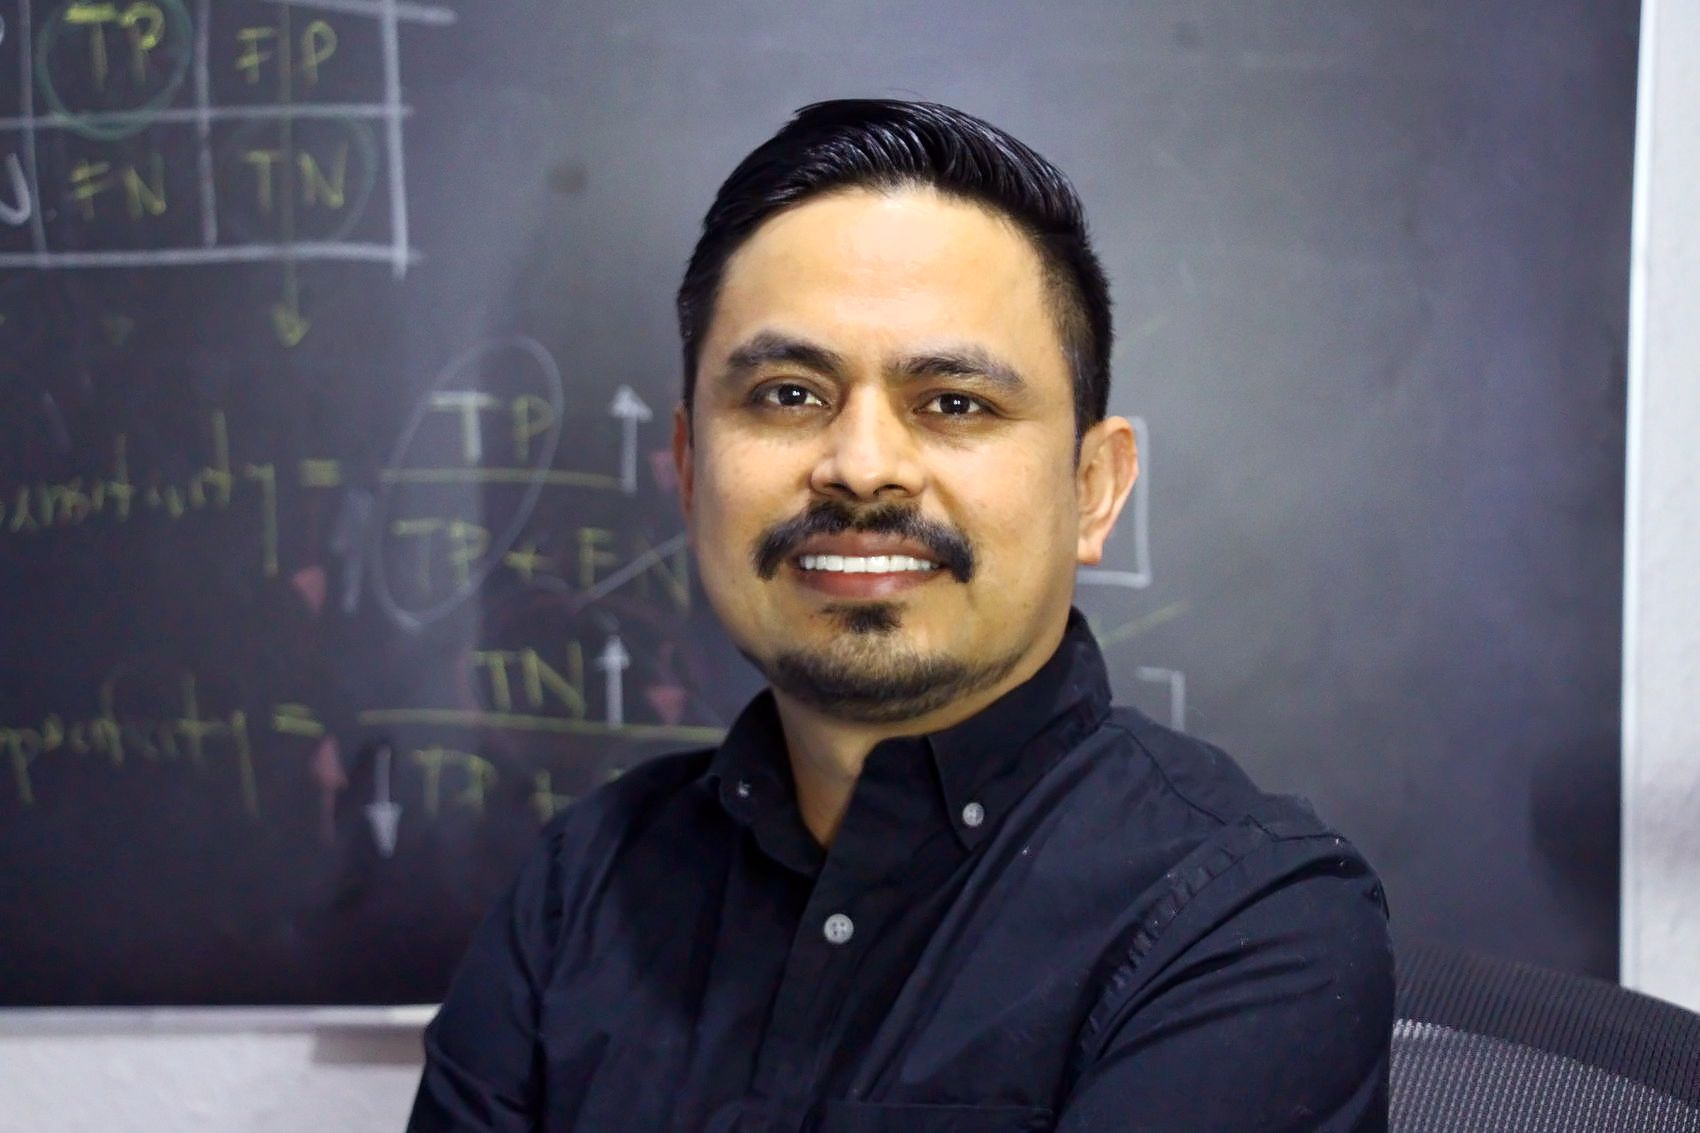
\includegraphics[width=0.3\linewidth]{24181AB1-FCDC-4431-9C59-D3C8CFDC3CAC}
	%	\caption{}
	%	\label{fig:24181ab1-fcdc-4431-9c59-d3c8cfdc3cac}
\end{figure}

\begin{itemize}
	\item Juan Irving Vasquez, PhD
	\item Centro de Innovación y Desarrollo Tecnológico en Cómputo (CIDETEC)
	\item Webpage: \url{jivg.org}
	\item \faIcon{envelope} jvasquezg@ipn.mx
	\item Tiktok irvingvasquez\_ia
	\item \faIcon{youtube} https://www.youtube.com/@IrvingVasquez
\end{itemize}
\end{frame}


\begin{frame}
	\frametitle{Curso}
	\begin{itemize}
		\item Redes neuronales y aprendizaje profundo
		\item Ingeniería en inteligencia artificial
		\item Temario oficial
		\url{https://www.escom.ipn.mx/docs/oferta/uaIIA2020/redesNeuronalesAprendizajeProfundo_IIA2020.pdf}
		\item Temario actualizado: %\url{https://jivg.org/courses/introduccion-a-las-redes-neuronales-2/}
		\item Calificación: 60\% tareas y exposiciones, 40 \% exámenes (3 exámenes)
		\pause
		\item Reglas internas:
		\begin{itemize}
			\item Los comunicados serán a través de teams
			\item No comer en el salón de clases
			\item Asistencia no tiene calificación
			\item Puntualidad
			\item No se permite el teléfono celular
			\item Deseable: no se permiten botellas desechables
		\end{itemize}
	\end{itemize}
\end{frame}


\begin{frame}
\frametitle{Bibliography}
\begin{itemize}
{\small 		
		\item Vasquez-Gomez, J.I. Introducción a las redes neuronales.
		\item Goodfellow, Ian, et al. Deep learning. Vol. 1. Cambridge: MIT press, 2016.
		\item Vishnu Subramanian, Deep Learning with PyTorch, 2018.
		\item Walpole, R. E., Myers, R. H., Myers, S. L., \& Ye, K. Probability and statistics for engineers and scientists (9th Ed). New York: Macmillan.
		\item Norvig, P., \& Russell, S. (2004). Inteligencia Artificial. Un Enfoque Moderno. Prentice Hall, Mexico.
		\item Skansi, S. (2018). Introduction to Deep Learning: from logical calculus to artificial intelligence. Springer.
		\item Scopatz, A. and Huff, K.D., 2015. Effective computation in physics: Field guide to research with python. " O'Reilly Media, Inc.".
		\item Kneusel, R.T., 2021. Math for deep learning: what you need to know to understand neural networks. No Starch Press.
}
\end{itemize}
\end{frame}

\begin{frame}
\frametitle{Recursos del curso}
\begin{itemize}
	\item \faIcon{github} Repositorio 1: \\ \url{https://github.com/irvingvasquez/cv2course_intro_nn}
	\item \faIcon{github} Reposotorio 2: \\ \url{https://github.com/irvingvasquez/practicas_pytorch}
	\item \faIcon{mobile-alt} Curso en línea: \\ \url{https://jivg.org/cursos/introduccion-a-las-redes-neuronales-2/}
	\item \faIcon{book} Juan Irving Vasquez, Introducción a las redes neuronales: libro de ejercicios.
	\url{https://github.com/irvingvasquez/libro_redes_neuronales}
\end{itemize}
\end{frame}


\begin{frame}
\frametitle{Requerimientos para el curso}
\begin{itemize}
	\item \faIcon{code} Programación en Python
	\begin{itemize}
		\item Programación orientada a objetos
		\item NumPy
		\item Pandas
		\item Pil
	\end{itemize}
	\item \faIcon{code} Ambientes de conda (COLAB), Kaggle
	\item \faIcon{pencil-alt} Algebra lineal
	\item \faIcon{pencil-alt} Probabilidad
	\item \faIcon{pencil-alt} Cálculo multivariable
	\item \faWrench \vspace{3pt} Libreta, lapiz, calculadora, tabla de derivadas.
\end{itemize}
\end{frame}


\begin{frame}
	\frametitle{Tareas}
	\begin{itemize}
		\item Se suben a través de teams. Durante el tiempo establecido. 
		\item Archivo PDF. Escaneado o exportado. Legible. Con nombre, fecha y número de ejercicio.
	\end{itemize}
%\begin{figure}
	\centering
	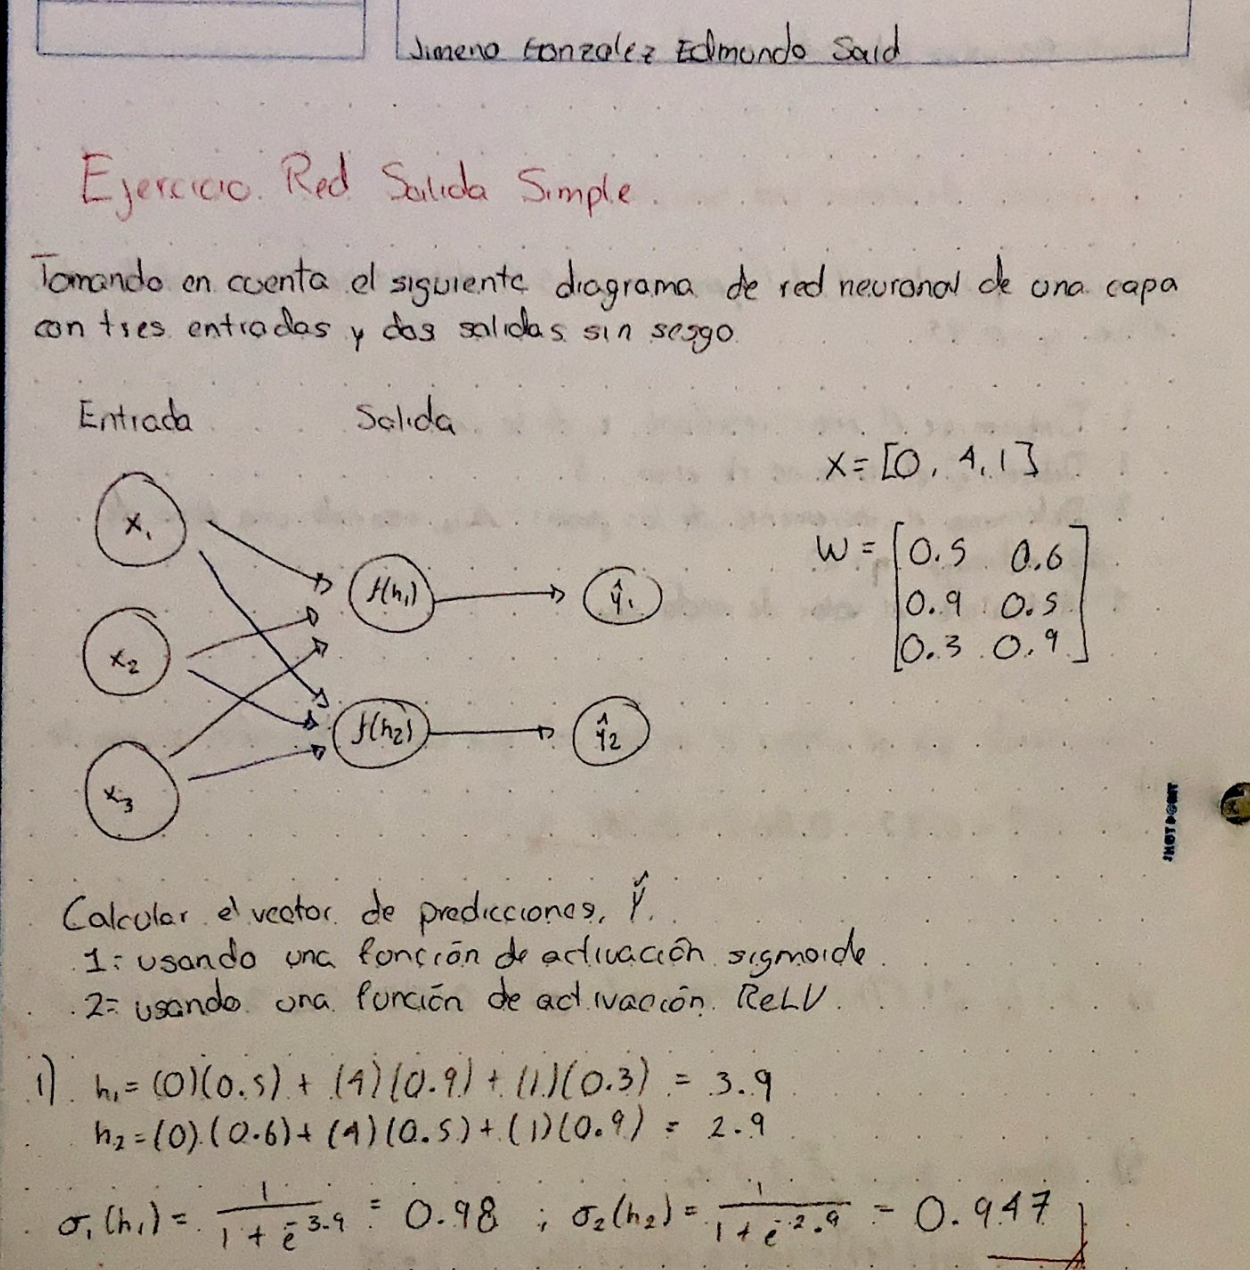
\includegraphics[height=0.8\textheight]{tareaeje}
	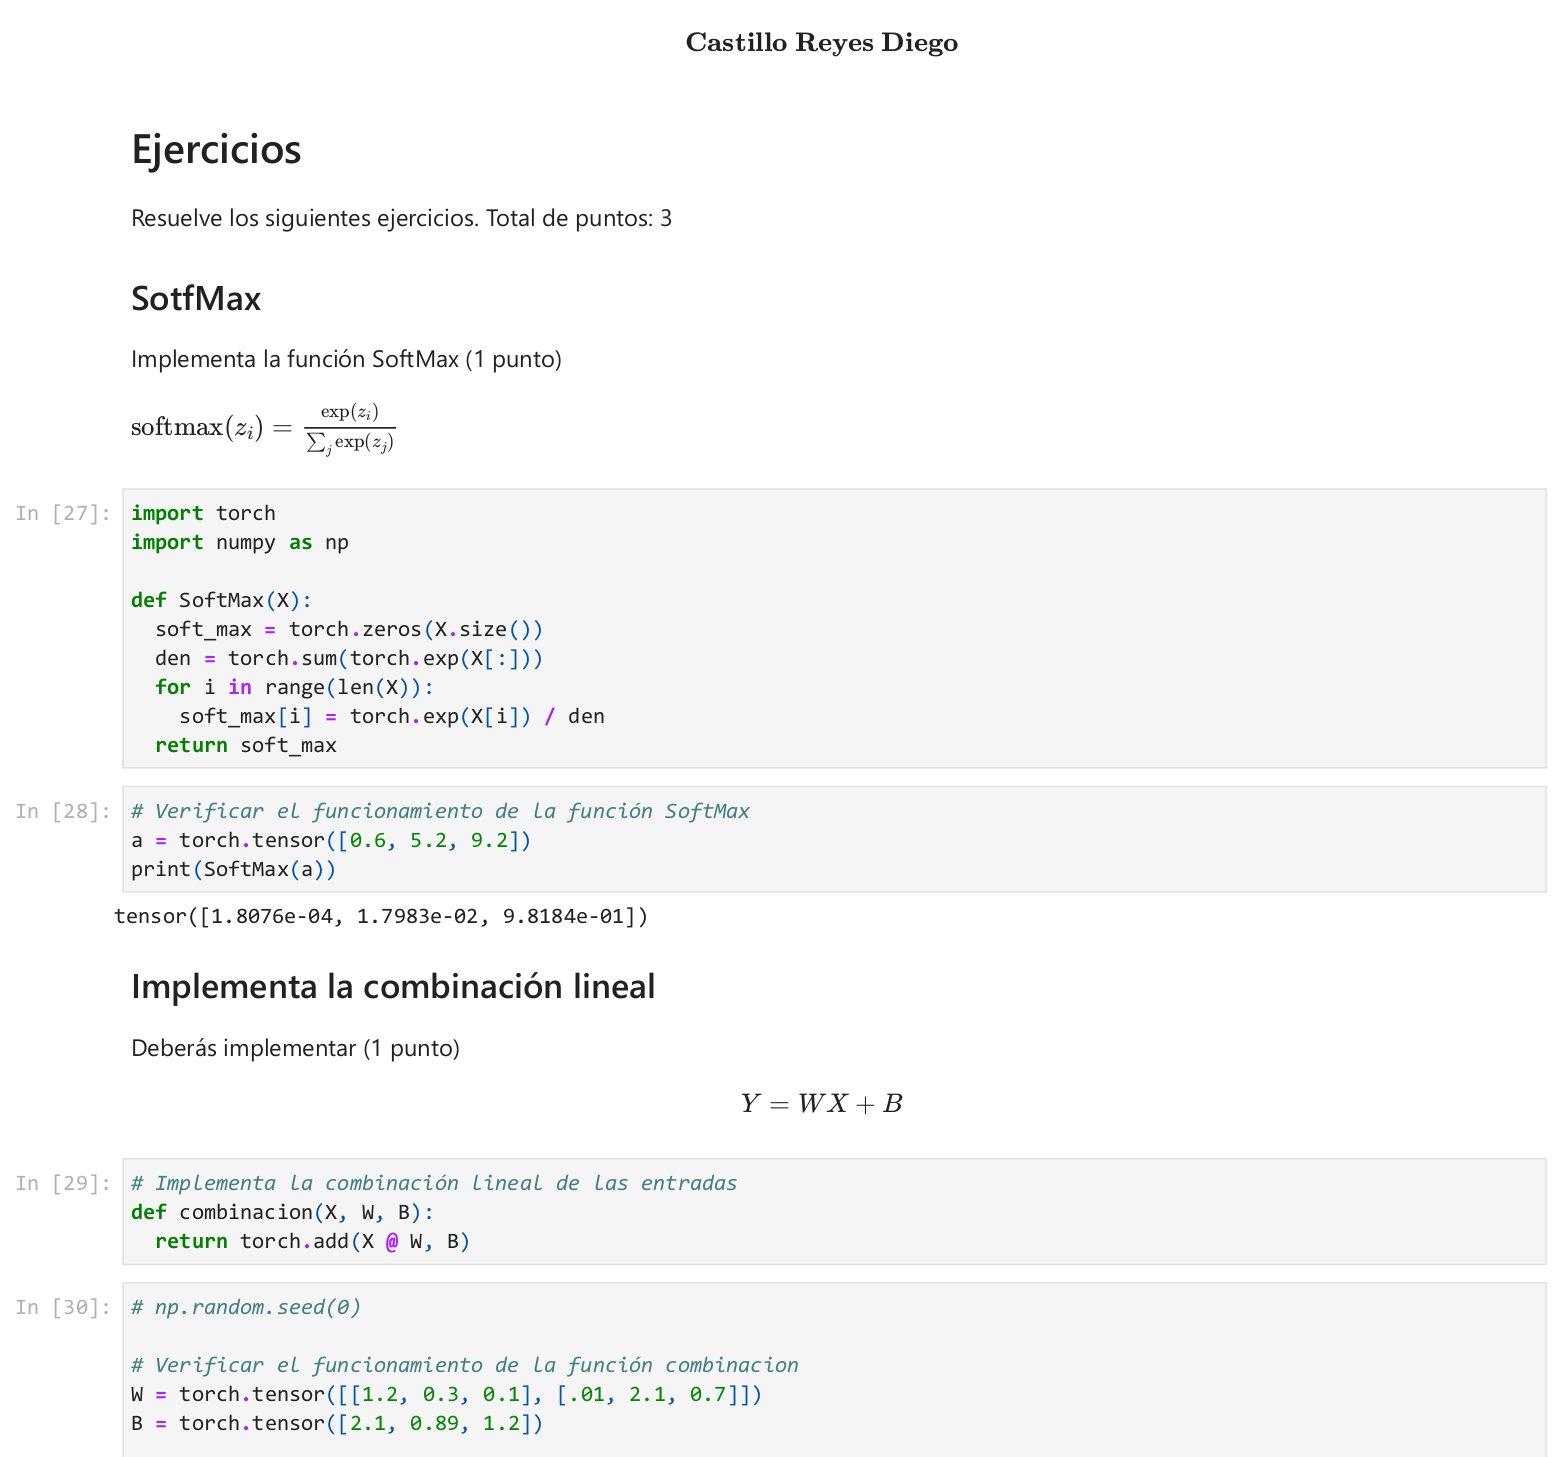
\includegraphics[height=0.8\textheight]{tareaprog}
%	\caption{}
%	\label{fig:tareaeje}
%\end{figure}

\end{frame}


\begin{frame}
	\frametitle{Lecturas para casa}
	\begin{itemize}
		\item Lecturas:
		\begin{itemize}
			\item Konstantino Kavafis, Ítaca
			\item 1.3 The history of artificial intelligence. Norvig and Russell.
			\item 18.8 Nonparametric models. Norvig and Russell.
			\item Prieto, R., Herrera, A., Pérez, L. and Padrón, A., 2000. El modelo neuronal de McCulloch y Pitts: Interpretación comparativa del modelo. UNAM.
		\end{itemize}
		\item Material adicional:
		\begin{itemize}
			\item Video: \url{https://youtu.be/0bMe_vCZo30?t=776}
		\end{itemize}
	\end{itemize}
\end{frame}


\begin{frame}
%	\frametitle{Sesión inaugural}
	\centering
	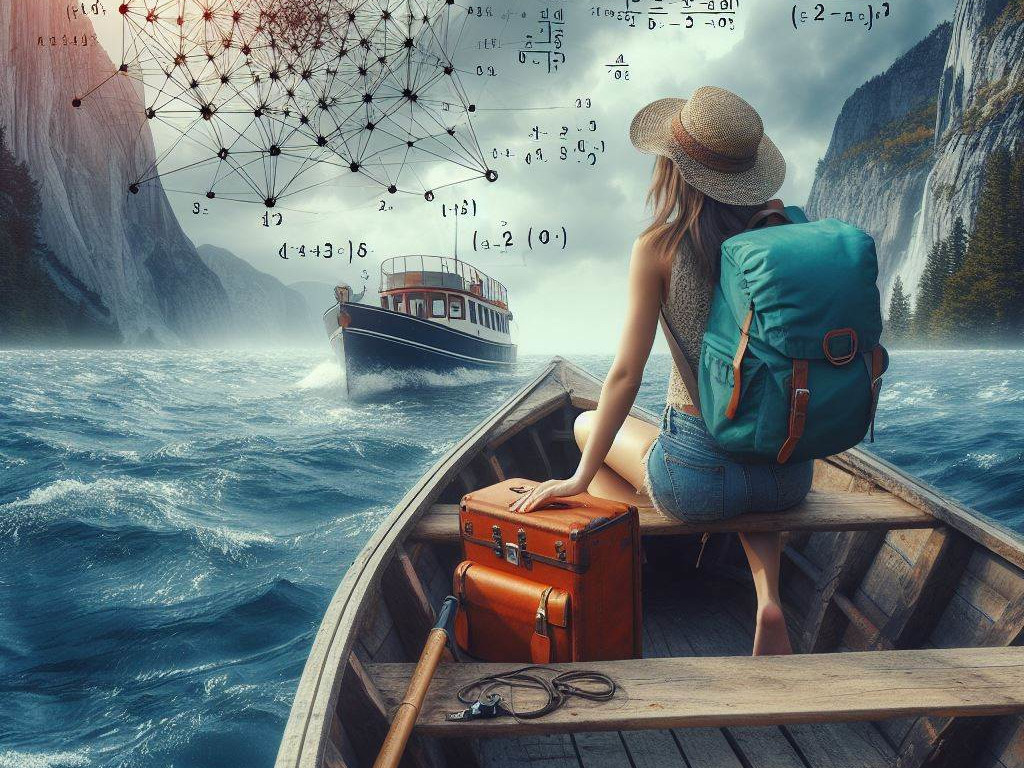
\includegraphics[width=0.9\linewidth]{itacaShort}
\end{frame}


%\begin{frame}
%\frametitle{Encuesta}	
%\begin{figure}
%	\centering
%	
\includegraphics[width=0.4\linewidth]{frame}
%	%\caption{}
%	%\label{fig:frame}
%\end{figure}
%\url{https://es.surveymonkey.com/r/BKR992P}
%\end{frame}




\end{document}